\subsection{Rotating Wave Approximation and Rabi oscillations}

We turn our attention now back to the full Hamiltonian of the problem. Let's re-write this equation in a more convinient way:

\begin{equation} \label{mod_ham}
    \hat{\mathcal{H}} = - \frac {\hbar \omega_{L}}{2} \hat{\sigma_{z}} - \frac {\hbar \Delta} {2} \hat{\sigma_{z}} + \hbar \Omega_{R} (e^{i\omega_{L}t} + e^{-i\omega_{L}t}) \hat{\sigma}_{x},
\end{equation}

where $\Delta = \omega_{a} - \omega_{L}$. Now we write down the transformation to the interaction picture with respect to the first term of expression \ref{mod_ham}, i.e. $\mathcal{H}_{0} = - \frac {\hbar \omega_{L}}{2}$.

Performing the transformation term by term, the first term is symmetrical under the this operation. We calculate then how $\hat{\sigma_{x}}$ transforms. Let's write $\hat{\sigma_{x}} = \hat{\sigma^{+}} + \hat{\sigma^{-}}$ and using the baker-Hausdorff lemma:

\begin{equation}
    e^{B}Ae^{-B} = B + [B,A] + \frac{1}{2!} [B, [B,A]] + ...,
\end{equation}

we find:

\begin{equation}
\begin{cases}
    \sigma^{+}_{I} = e^{ i \omega_{L}t} \sigma^{+} \\
    \sigma^{-}_{I} = e^{ - i \omega_{L}t} \sigma^{-}
\end{cases}
\end{equation}

Writing the interaction Hamiltonian in the interaction picture like:

\begin{equation}
    \mathcal{H}_{int}^{I} = - \hbar \frac{\Delta}{2} \hat{\sigma_{z}} + \hbar\Omega_{R} (e^{i \omega_{L} t} + c.c.) (e^{i \omega_{L} t} \hat{\sigma}^{+} + e^{-i \omega_{L} t}\hat{\sigma}^{-})
\end{equation}

In this expression some terms do not oscillate and other oscillate with $2\omega_{L}$. The rotating wave approximation consists in neglecting those fast oscillating terms. The interaction then is finally written:

\begin{equation} \label{h_int}
    \mathcal{H}_{int}^{I} = - \hbar \frac{\Delta}{2} \hat{\sigma_{z}} + \hbar\Omega_{R} \hat{\sigma}_{x}
\end{equation}

In the matrix form, in units of $\hbar$:

\[
\mathcal{H}_{int}^{I} =
  \begin{bmatrix}
    - \Delta / 2 & \Omega_{R}  \\
    \Omega_{R} & \Delta / 2
  \end{bmatrix}
\]

We can apply the same transformation again with respect the $\sigma_{z}$ part of this new Hamiltonian to solve the problem. We already knowhow $\sigma_{x}$ transforms: $\mathcal{H}_{I} = \Omega_{R} (e^{i\Delta t} \sigma^{+} + e^{-i\Delta t} \sigma^{-})$.
Inserting this operator in the TDSE in the interaction picture we find:

\begin{equation} \label{coupled_equations}
\begin{cases}
    i \dot{c}_{0}(t) = \Omega_{R} c_{1}(t) e^{-i \Delta t} \\
    \\
    i \dot{c}_{1}(t) = \Omega_{R} c_{0}(t) e^{i \Delta t},
\end{cases}
\end{equation}
which leads, for the excited state, a general function of the type:

\begin{equation} \label{c1}
    c_{1}(t) = A e^{i\Delta t / 2}(e^{i\Omega't/2} - e^{-i\Omega't/2}),
\end{equation}

with $\Omega' = \sqrt{\Delta^{2} + 4 \Omega_{R}^{2}}$. This expression was written by having in mind the initial condition $|c_{1}(t=0)|^{2} = 0$, but that is not enough the determine $A$. To determine this coefficient we insert \ref{c1} in the coupled differential equations \ref{coupled_equations}, calculate $c_{0}(t)$ and consider $|c_{0}(t=0)|^{2} = 1$, which fully determines $A$:

\begin{equation}
    \begin{cases}
    |c_{1}(t)|^{2} = \frac{4\Omega_{R}^{2}}{\Delta^{2} + 4 \Omega_{R}^{2}} \frac{1}{2}(1 - \textrm{cos} \Omega't) \\
    \\
    |c_{0}(t)|^{2} = \frac{\Delta^{2}} {\Omega'^{2}} \textrm{sin}^{2}(\Omega't/2) + \textrm{cos}^{2}(\Omega't/2)
    \end{cases}
\end{equation}

And the complete wavefunction:

\begin{equation}
    \ket{\psi} = - e^{-i\Delta t/2}[\textrm{cos}(\Omega't/2) + i \frac{\Delta}{\Omega'} \textrm{sin}(\Omega' t /2)] \ket{0} + i \frac{2\Omega_{R}}{\sqrt{\Delta ^{2} + 4\Omega_{R}^{2}}} e^{i\Delta t / 2} \textrm{sin}(\Omega' t / 2) \ket{1}
\end{equation}

The on resonance case $\Delta=0$, flips the population entirely from the ground state to the excited state when the atoms are illuminated with a pulse duration $t_{\pi}$, where $2\Omega_{R}t_{\pi} = \pi$. This is traditionally called a $\pi$--pulse. On figure \ref{rabi_osc} the several cases of pulse duration and detuning are plotted. It is important to note that the $\pi$--pulse value is representative of the dipole matrix connecting the ground and excited states and the laser intensity. Therefore, it is a special property of the atom----laser interaction. Indeed:

\begin{equation}
    \begin{cases}
        \Omega_{R} = \frac{e\mathcal{E}_{0}}{2\hbar} \bra{1} \vec{r} \cdot \hat{\epsilon} \ket{0} \\
        \\
        t_{\pi} = \frac{\pi}{2\Omega_{R}}
    \end{cases}
\end{equation}

\begin{figure}[h]
\centering
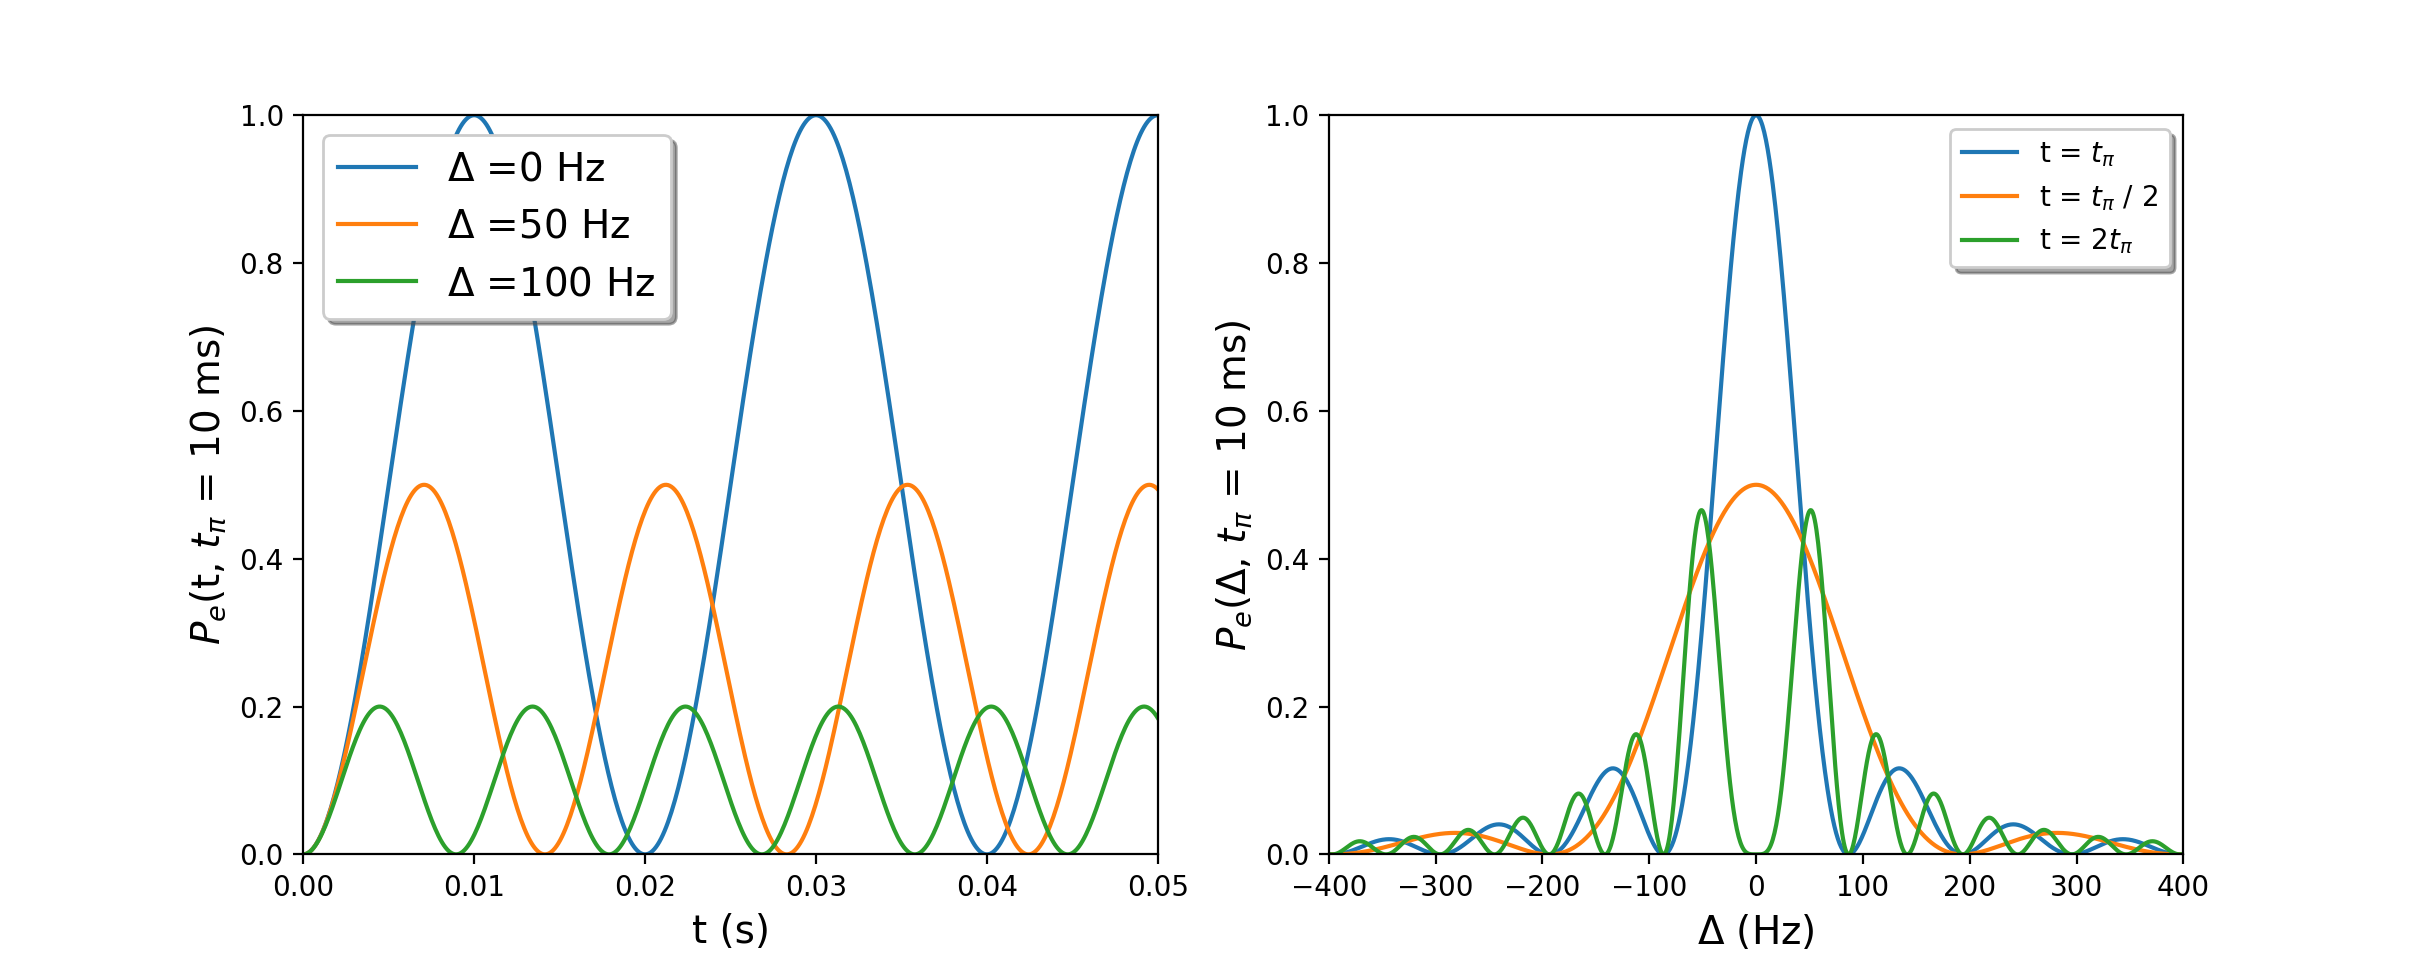
\includegraphics[width=\linewidth]{./plots/Rabi_Oscillations/rabi.png}
\caption{On the right--hand figure it is plotted the transition line shape as a function of the laser detuning from the atomic resonance for different pulse durations. Fixing now the laser frequency with a certain detuning and varying the interaction time or pulse duration, yields to the plot on the left--hand side.}
\label{rabi_osc}
\end{figure}

As you can guess, in the experiment, there are only two parameters that the experimentalist will be interested in to characterize or set up the experiment: $t_{\pi}$ (or the laser intensity) and $\Delta$. It is useful then to re-write the expression for the population of the excited state as a function of these two parameters:

\begin{equation}\label{p_excited}
    P_{e}(t, \Delta) = \left(\frac{\pi}{2}\right)^{2} \left( \frac{ \textrm{sin}\Delta' t/t_{\pi}} {\Delta'} \right)^{2},
\end{equation}

with $\Delta' = \frac{\pi}{2} \sqrt{1 + (t_{\pi} \Delta / \pi)^{2}}  $.

A useful relation is to calculate the Full Width Half Maximum (FWHM) when the laser pulse duration is set to $t_{\pi}$. Defining $P_{e}(t=t_{\pi}, \Delta=\delta/2) = 0.5$ and inserting this in equation \ref{p_excited} we find the equation to solve:
\begin{equation}
    \textrm{sin}\Delta' = \frac{\sqrt{2}\Delta'}{\pi}
\end{equation}
Expanding the sine function we find:
\begin{equation} \label{sinc}
    \begin{cases}
    \sum_{k=0}^{\infty} \frac{(-1)^{k}\Delta'^{2k}}{(2k+1)!} - \frac{\sqrt{2}}{\pi} = 0 \\
    \\
    t_{\pi}\delta = \sqrt{ (\frac{2\Delta'}{\pi})^{2} - 1}
    \end{cases}
\end{equation}

Truncating the series up to $k=3$, we find $t_{\pi}\delta \approx 0.797$, with $\delta$ in Hz. This simple numerical relation tells us that the width of the resonance shape is inversely proportional to the laser pulse duration. Hence, if you are seeking to observe a very narrow atomic resonance using the Rabi spectroscopy scheme (using a $\pi$-pulse to flip the atomic population), the pulse duration may represent a limitation for how narrow the observed transition can be, and in general, this yields in a technical limitation for the precision of experiments.

In the context of optical clocks, where the natural line width of the clock resonances are sub-Hertz, the Rabi profile is the observed resonance shape, limiting the stability of the clocks. The general pratice is then to set $t_{\pi}$ as long as possible. The superior technical limit for the pulse duration is naturally the coherence time of the laser, which, by Fourier transform, is related to the clock laser frequency fluctuations or phase noise. A standard practice is to reference the clock laser to an Ultra Stable Cavity (USC) with a finesse on the order of hundreds of thousands.
The ultimate limit then becames the brownian motion of the cavity mirror coating or thermal agitation, producing a noise in the cavity length and hence noise in the resonance frequency of the cavity which propagates to the laser stabilized to cavity. Solutions to this problem include cryogenic USC and long distance between the mirrors. The coherence time of clock lasers is typically near 1 second.

We quick calculate of the laser line width based on the coherence time of the laser by measuring the longest $t_\pi$ that we can set in the experiment. Let's suppose the ideal case when the laser is turned on at $t=-t_{\pi}/2$ and off at $t=t_{\pi}/2$. First step is to calculate the Fourier frequencies associated with this pulse:

\begin{equation}
    \begin{split}
        \mathcal{F}[\mathcal{E}(t)] & = \int^{\infty}_{-\infty} \mathcal{E}(t) e^{-i\omega t} dt \\
        & = \int^{t_{\pi}/2}_{-t_{\pi}/2} \mathcal{E}_{0} e^{-i\omega t} dt \\
        & = \mathcal{E}_{0} t_{\pi} \frac{\textrm{sin} (\omega t_{\pi}/2)} {\omega t_{\pi}/2}
    \end{split}
\end{equation}

Now we calculate the width of this profile in the exact same way as in equations \ref{sinc}. This leads to an approximate result:

\begin{equation}
    \Delta \nu _{FWHM} \approx \frac{1.2}{t_{\pi}}
\end{equation}

Hence, for a 1 second coherence time, the laser has an approximate line width of 1.2 Hz, according to this model. From this we conclude that to observe sub-Hertz atomic resonances, laser coherence times longer than 1 s is required.